
\documentclass[conference]{IEEEtran}

\usepackage{float} 
\usepackage{url}  
\usepackage{multirow}
\usepackage{caption}
\usepackage{subcaption}
\usepackage{booktabs}
\usepackage{cite}
\pagestyle{plain}
\usepackage{amsmath}
\usepackage{float}
\usepackage{tikz}
\usetikzlibrary{shapes.geometric, arrows, positioning}
\usepackage{placeins}
\usepackage{comment}
\usepackage{tabularx}
\ifCLASSINFOpdf
  \usepackage[pdftex]{graphicx}
\fi

\hyphenation{op-tical net-works semi-conduc-tor}

\begin{document}


\title{Exploring financial sentiment analysis with the Financial Phrasebank dataset}

\author{\IEEEauthorblockN{\\ Hugo Veríssimo}
\IEEEauthorblockA{Complements of Machine Learning 24/25\\
University of Aveiro\\
Aveiro, Portugal\\
hugoverissimo@ua.pt}
\and
\IEEEauthorblockN{\\ João Cardoso}
\IEEEauthorblockA{Complements of Machine Learning 24/25\\
University of Aveiro\\
Aveiro, Portugal\\
joaopcardoso@ua.pt}}

\maketitle
\thispagestyle{plain}

\begin{abstract}
abstratotoototot
\end{abstract}

\begin{quote}
\small
\noindent
\textbf{Keywords:} key, word, number, 1
\end{quote}

\IEEEpeerreviewmaketitle


\section{Introduction}

With the ever increasing volume of information created and distributed by the minute, it is more important than ever to have access to fast and reliable analysis of any information we may come across. Especially with the democratized access to financial instruments and capital markets, where individuals have the possibility to invest in virtually any company on the stock exchange, it is important to have ways to leverage against giant institutions with hundreds of financial analysts at their disposal. 

\begin{figure}[H]
    \centering
    
\includegraphics[width=0.5\linewidth]{bugs.png}
    \caption{Power to the people, colorized (circa 1917).}
    \label{fig:enter-label}
\end{figure}

Historically, financial analysis relied heavily on fundamental analysis (examining earnings, balance sheets, annual financial reports), which required extensive knowledge in the field (also the strategy that made Warren Buffett one of the richest men in the world), along with technical analysis (studying price and volume trends). Around 2010, after the 2008 global financial crisis, there was a surge in news analysis to evaluate the tone and derive investment strategies from it. Due to the lack of domain specific lexicon these analysis were falible, until the work by Loughran and McDonald was published, a financial lexicon based on 10-K forms (i.e., annual financial reports) and dictionaries. This allowed to use more sofisticated analysis rather than using the presence of negative words as a signal to sell.

Upon the launch of Twitter, information streams increased dramatically, making more and more data available for analysis. But, machine learning was not heavily used, as most data was not annotated, or there was very little data with high-quality annotations. In 2014, P. Malo \textit{et al.} published a fundamental dataset for financial sentimental analysis, that is still used, the Financial Phrasebank. It is unique, for the inclusion of important aspects as directional expressions (e.g., profits decreased), entity polarity shifts (e.g. profits may be negative if decreased), and phrase level context.

With this, machine learning models started finding their place in research, as the field of natural language processing grew and niche fields such as financial investments found useful data. In this work we explore the Financial Phrasebank dataset, by implementing different machine learning and deep learning models.

\section{State of The Art}



\section{Methodology}

\subsection{Dataset \& EDA}

The Financial PhraseBank is a widely used benchmark dataset for financial sentiment analysis. It consists of roughly 4,840 English sentences (mostly news headlines or short statements) about companies, drawn from financial news articles and press releases. Each sentence is labeled with one of three sentiment classes – positive, negative, or neutral – representing the sentence’s sentiment from the perspective of an investor.

+ 50 66 75 percento

ns q concordancia bla bla

https://huggingface.co/datasets/takala/financial\_phrasebank
\cite{dataset, malo2013gooddebtbaddebt}


\subsection{Preprocessing}

split teste e treino

\section{Models}

abcbdhdhhd

\subsection{model 1}

model 1


\subsection{model 2}

model 2

\subsection{model 3}

model 3

\section{Exploring BERT}

\subsection{base model}

\begin{table}[H]
\centering
\caption{Hyperparameter space for ......}
\label{parameters_basebert}
\begin{tabular}{ll}
\toprule
\textbf{Hyperparameter} & \textbf{Possible Values} \\
\midrule
Epochs & $\{1,2,3,4,5\}$ \\
Learning rate & $[10^{-5}, 10^{-2}]$ \\
Weight decay & $[0, 0.5]$ \\
\bottomrule
\end{tabular}
\end{table}

best hyperameters: 

- Num train epochs: 2.0

- Learning rate: 0.0001

- Weight decay: 0.1

\begin{figure}[H]
    \centering
    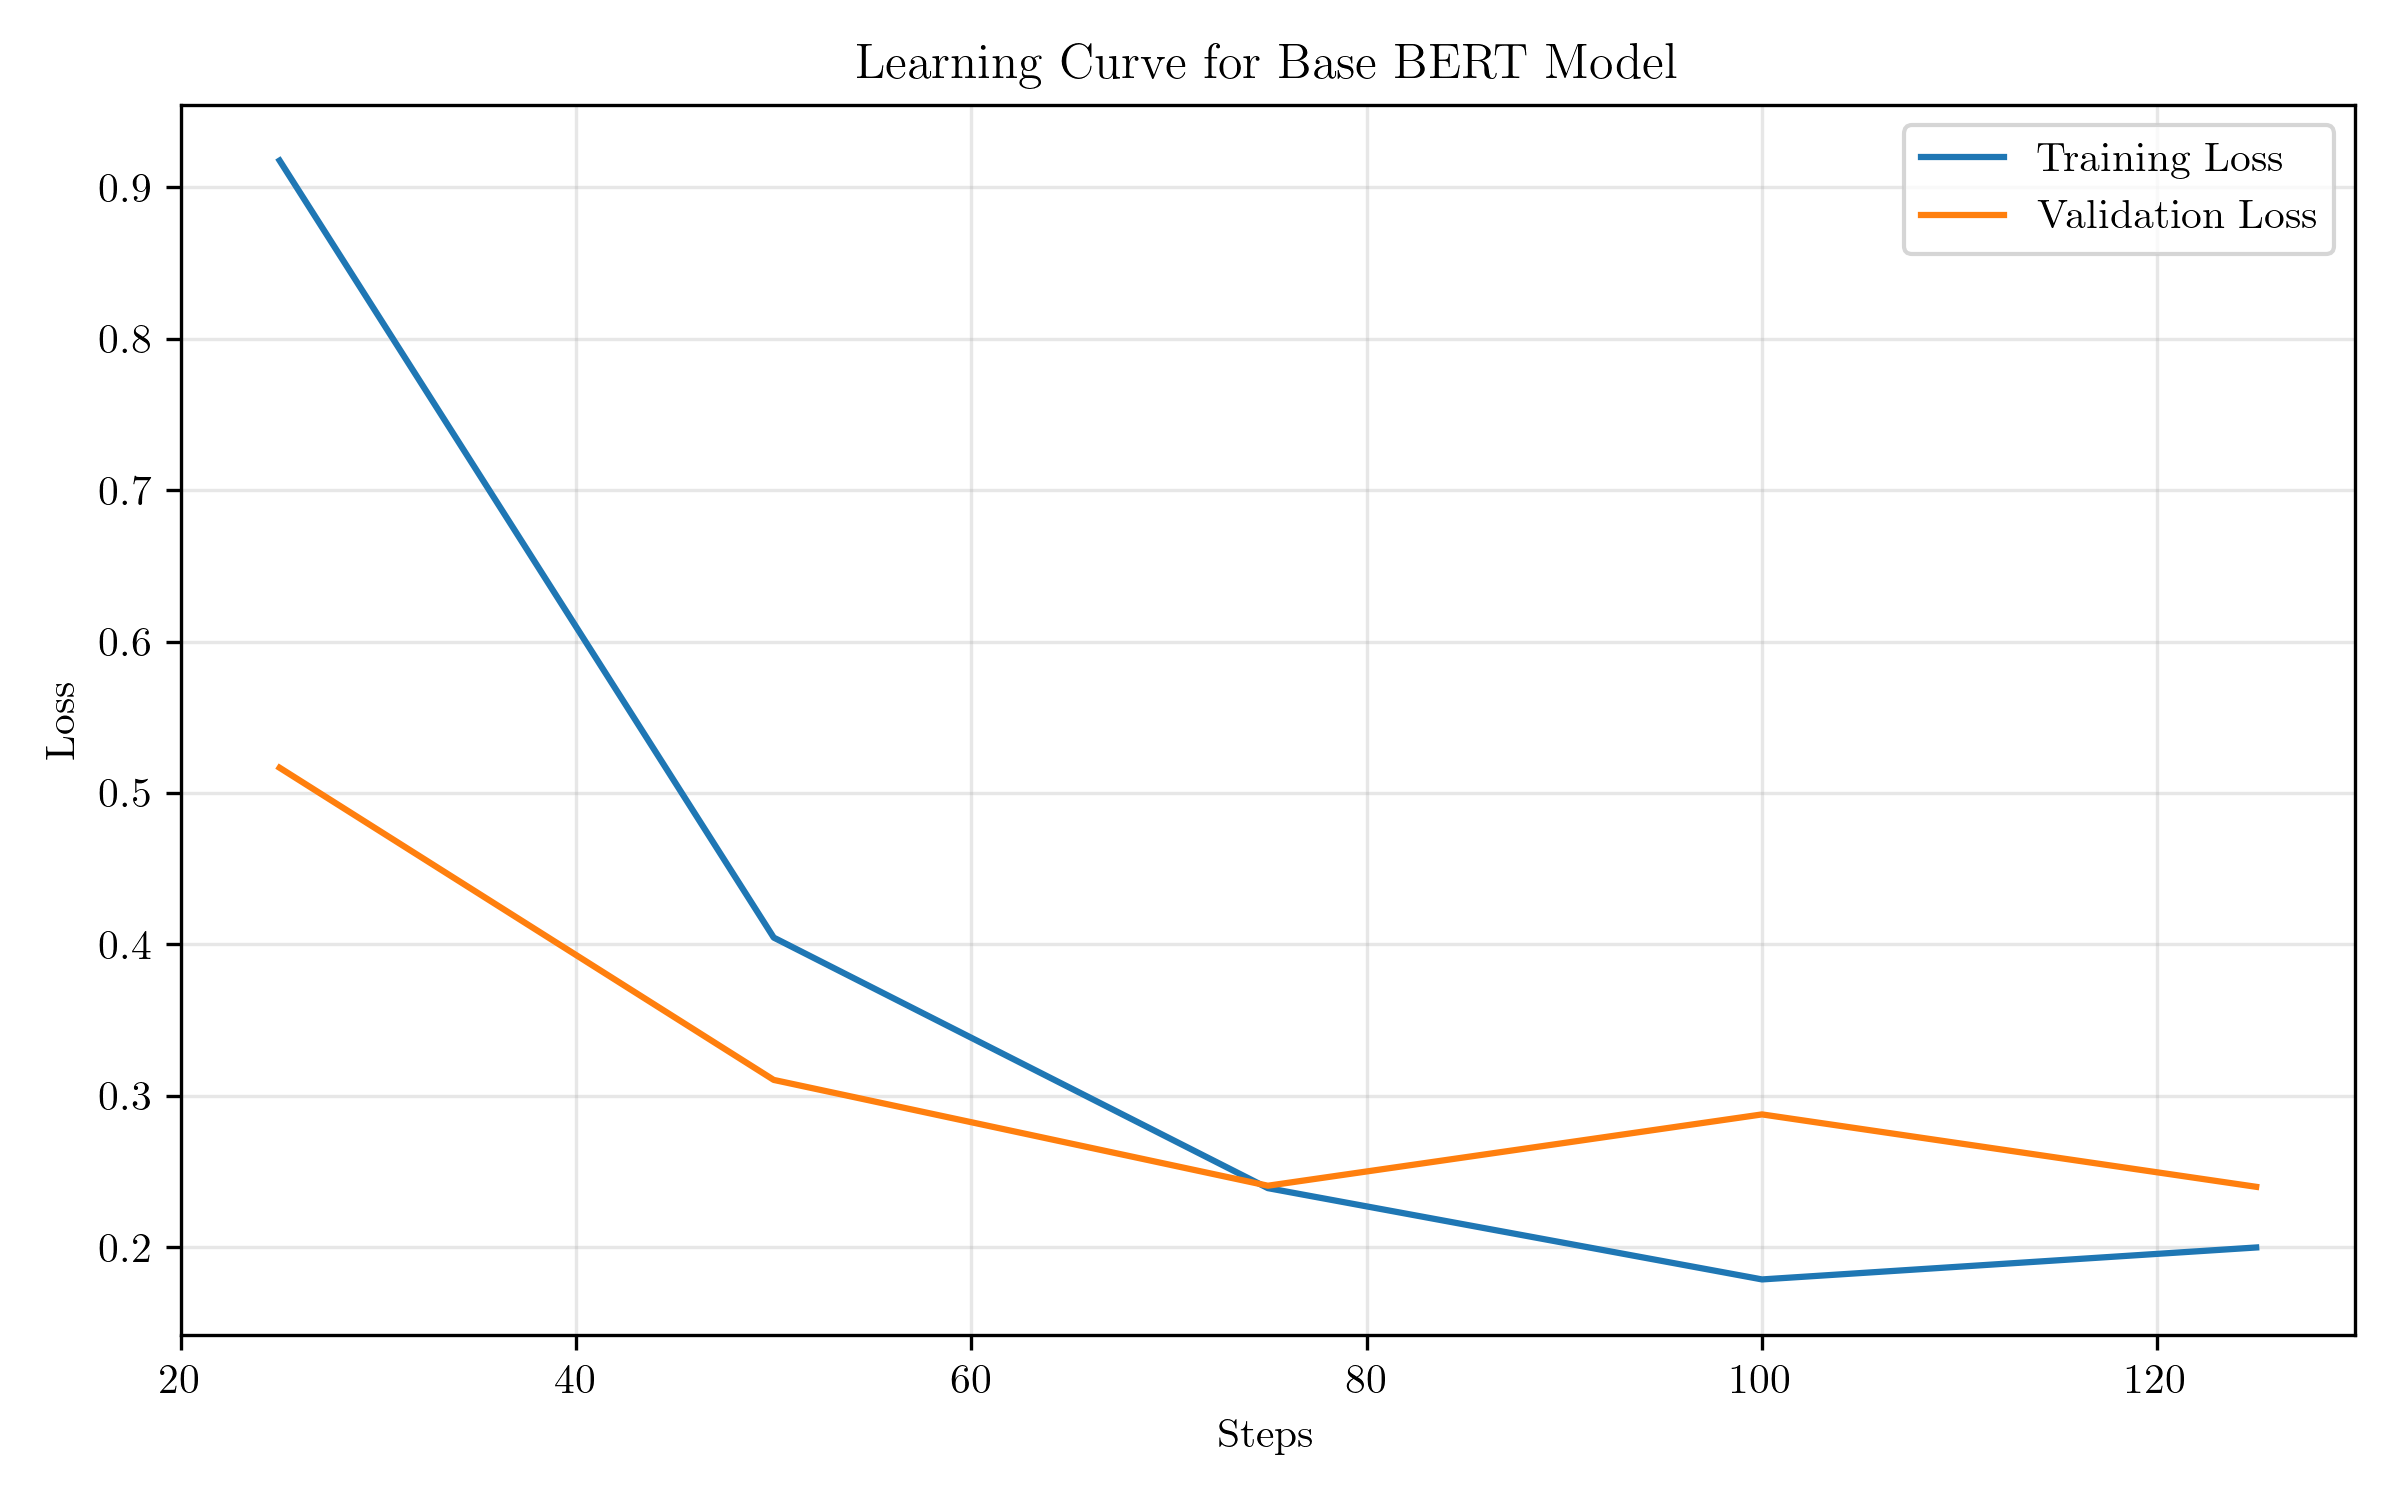
\includegraphics[width=1\linewidth]{assets/base_bert_learning_curve.png}
    \caption{learning curve}
    \label{fig:base_bert_learning_curve}
\end{figure}

\begin{figure}[H]
    \centering
    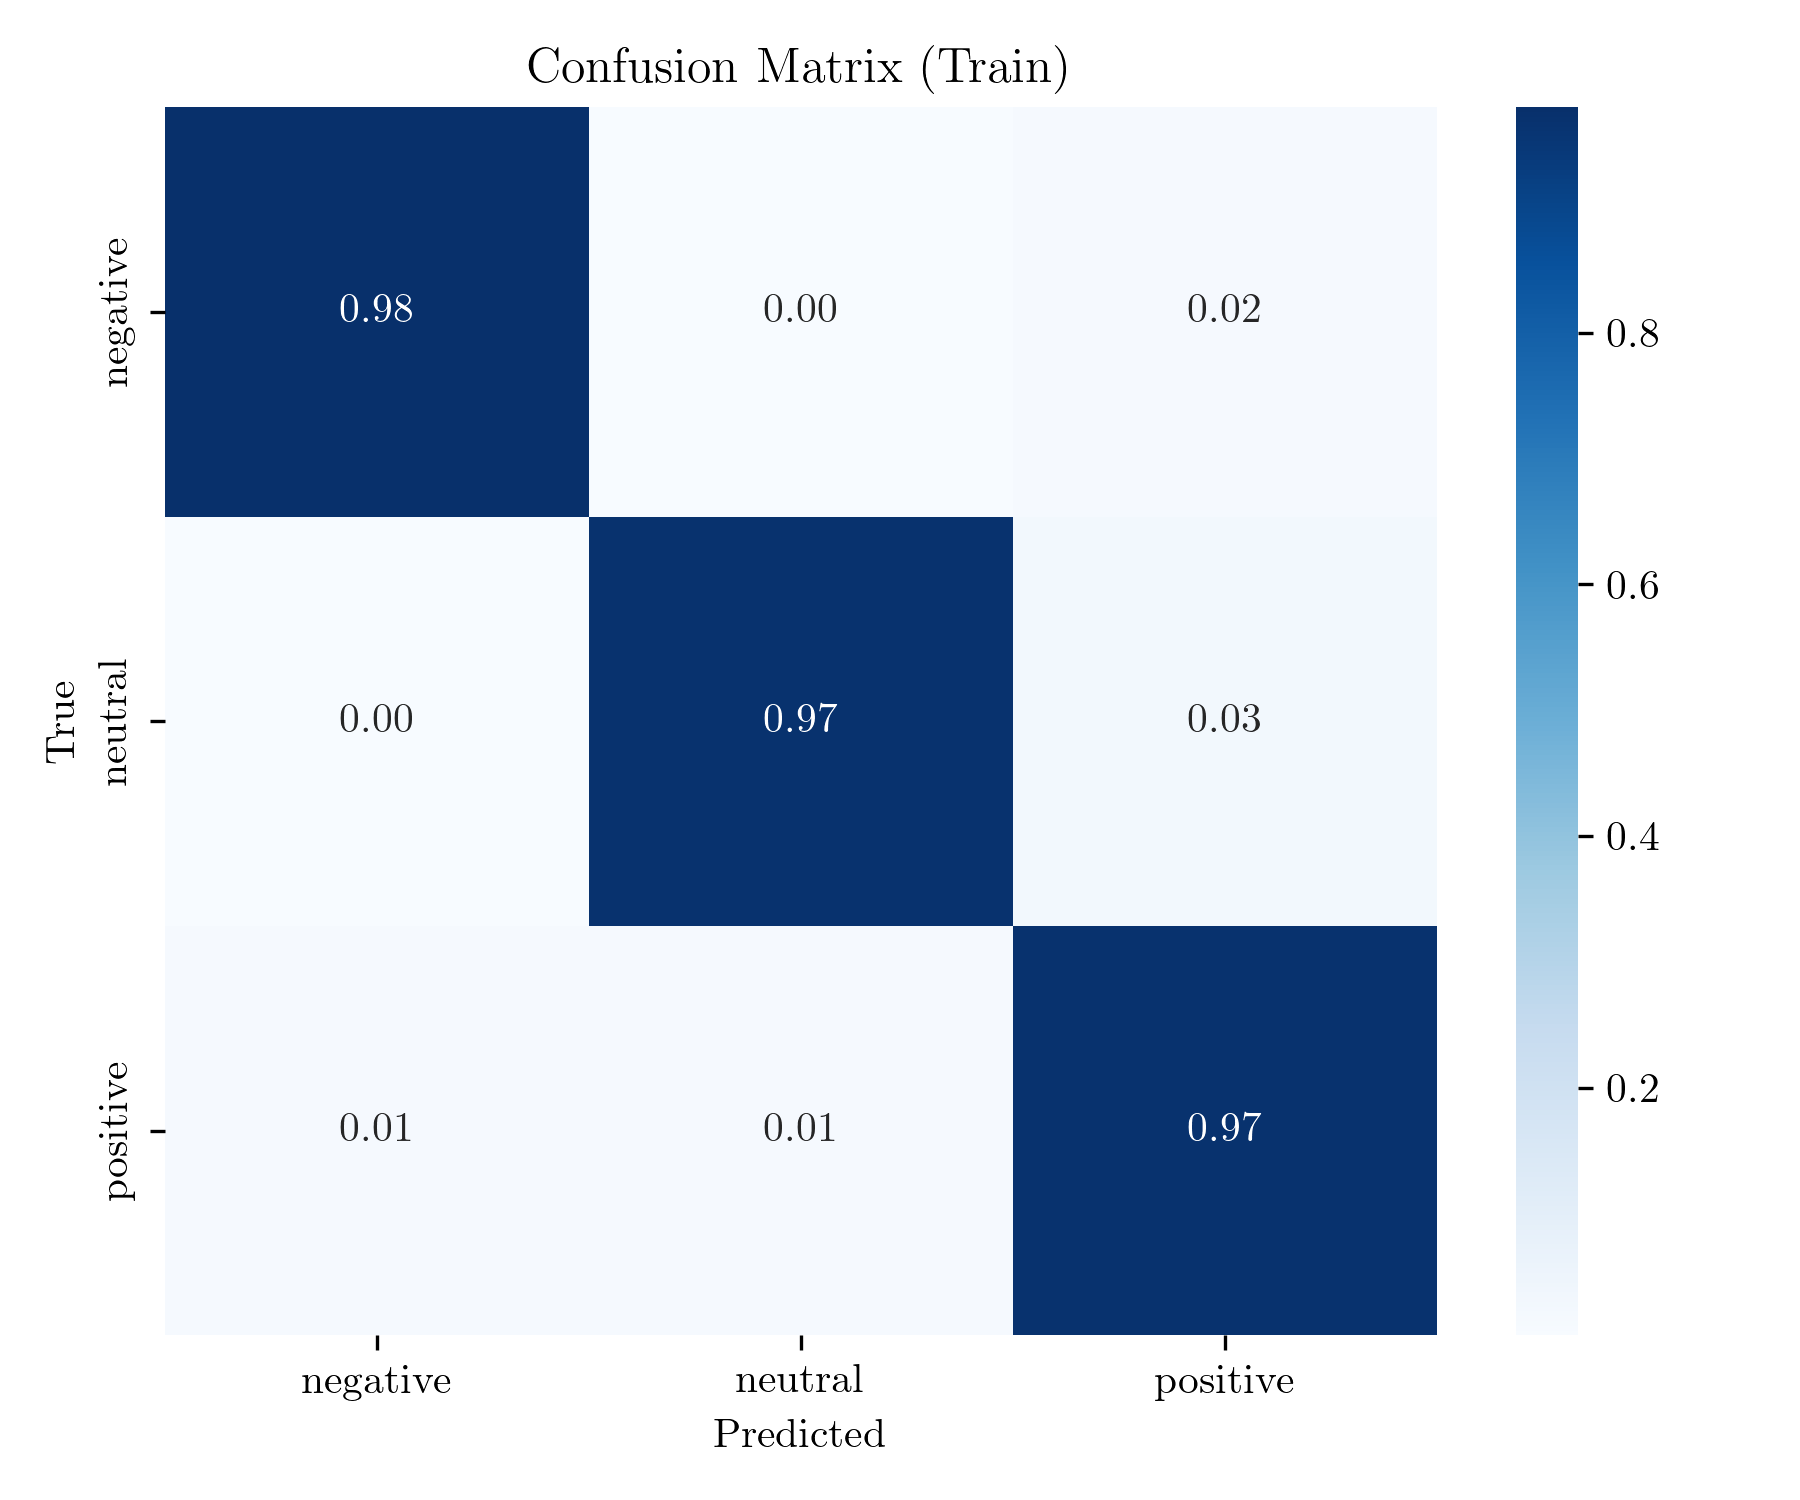
\includegraphics[width=1\linewidth]{assets/base_bert_confusion_matrix_Train.png}
    \caption{base bert conf matri train}
    \label{fig:base_bert_confusion_matrix_Train}
\end{figure}

\begin{table}[H]
\centering
\caption{Classification report for BASE BERT on training data.}
\label{cr_basebert_train}
\begin{tabular}{lcccccc}
\toprule
\textbf{Class} & \textbf{Precision} & \textbf{Recall} & \textbf{F1-Score} & \textbf{Support} \\
\midrule
Negative & 0.98 & 0.98 & 0.98 & 336 \\
Neutral & 0.98 & 0.97 & 0.98 & 336 \\
Positive & 0.96 & 0.97 & 0.96 & 336 \\
\midrule
\textbf{Accuracy} &  &  & 0.97 & 1008 \\
\textbf{Macro avg} & 0.97 & 0.97 & 0.97 & 1008 \\
\textbf{Weighted avg} & 0.97 & 0.97 & 0.97 & 1008 \\
\bottomrule
\end{tabular}
\end{table}

\begin{figure}[H]
    \centering
    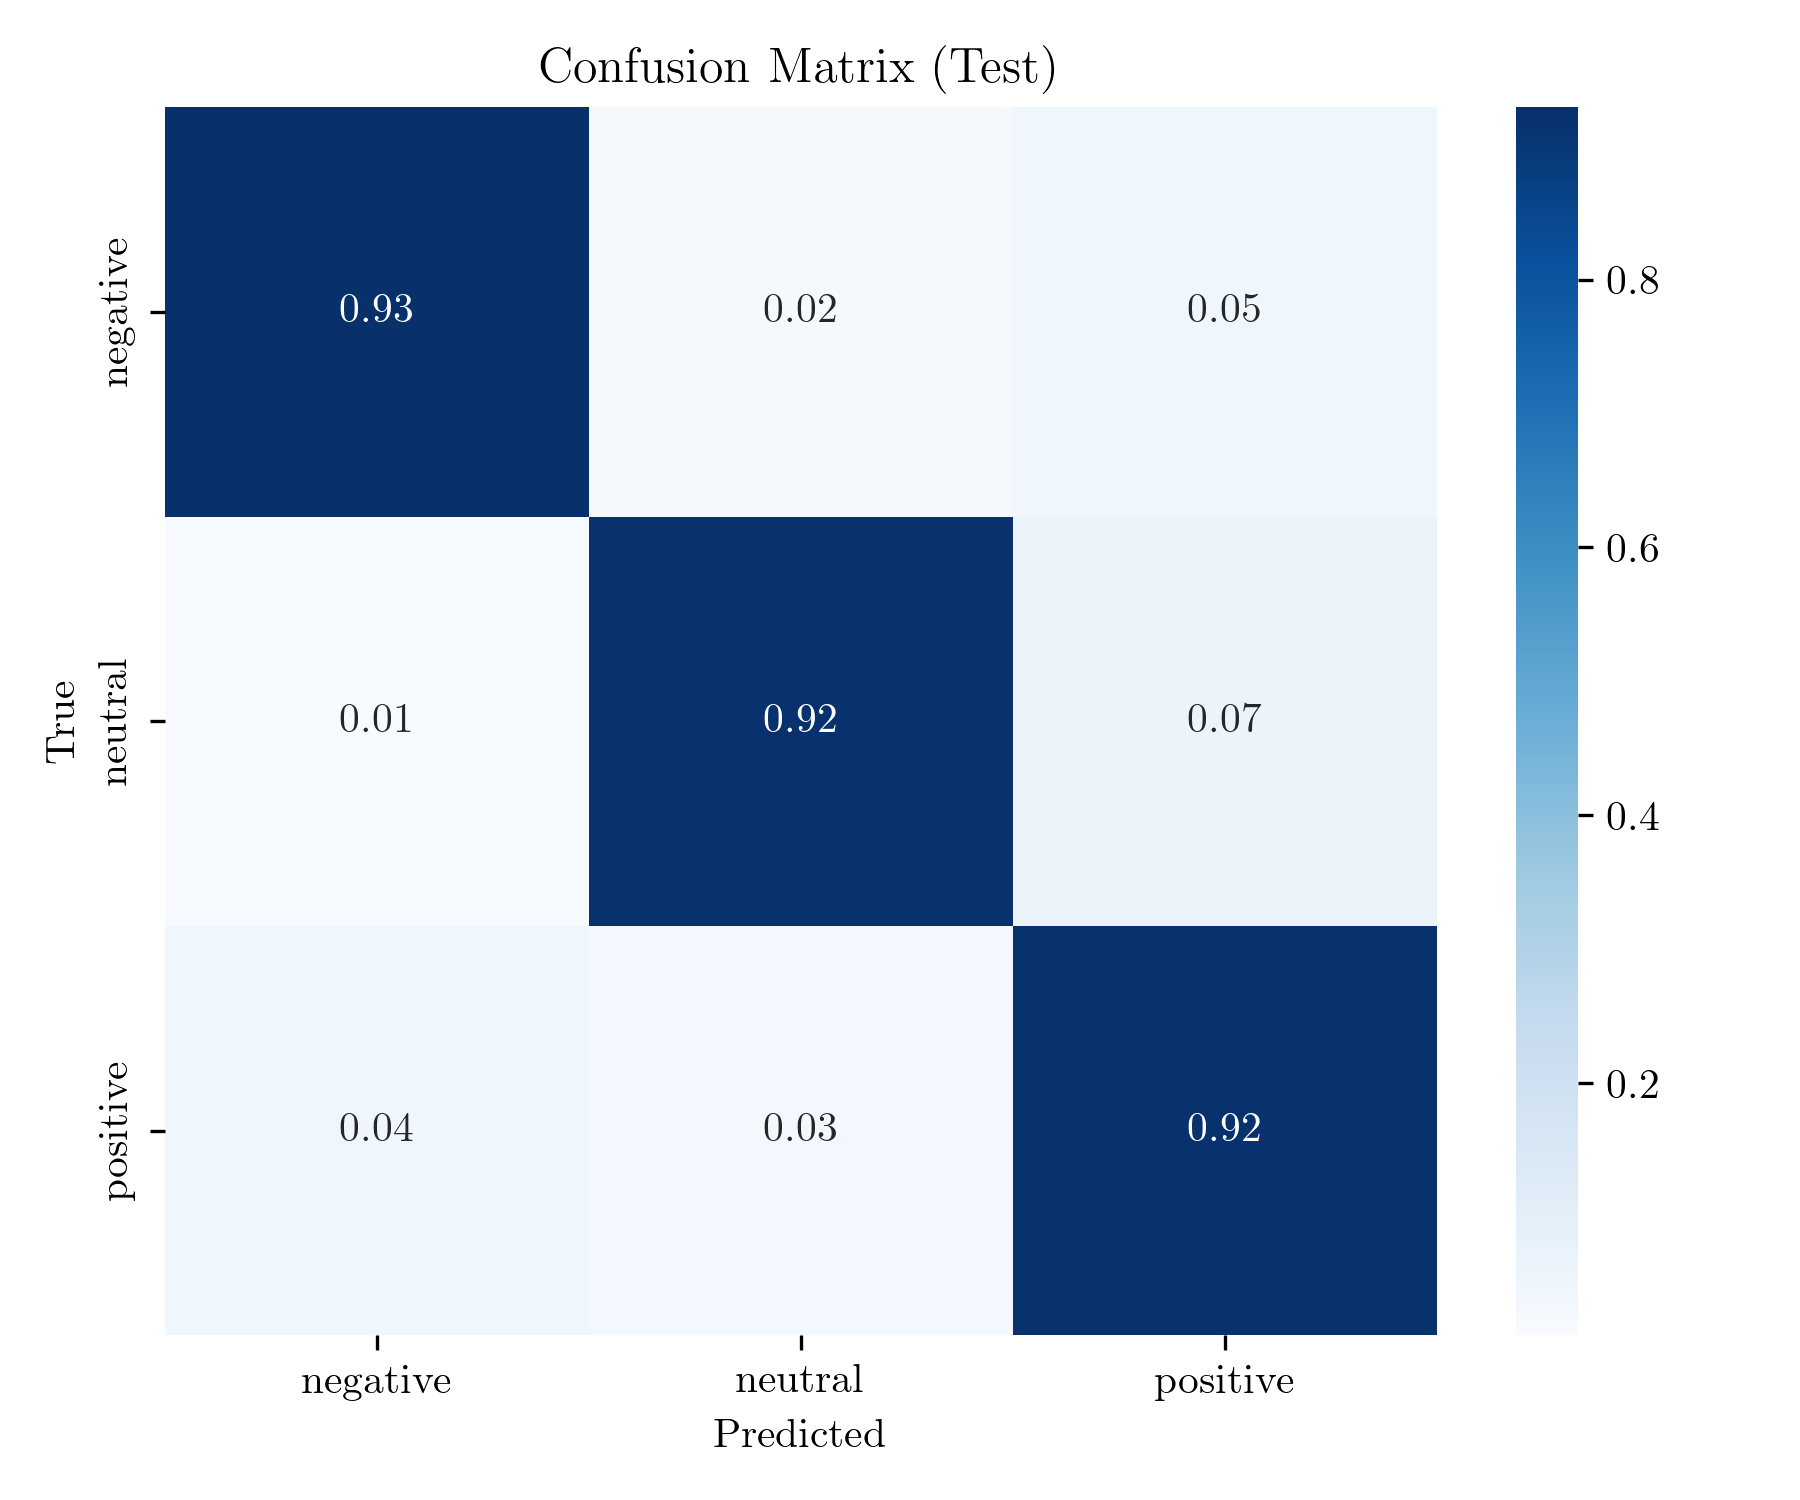
\includegraphics[width=1\linewidth]{assets/base_bert_confusion_matrix_Test.png}
    \caption{base bert cong matrix test}
    \label{fig:base_bert_confusion_matrix_Test}
\end{figure}

\begin{table}[H]
\centering
\caption{Classification report for BASE BERT on test data.}
\label{cr_basebert_test}
\begin{tabular}{lcccccc}
\toprule
\textbf{Class} & \textbf{Precision} & \textbf{Recall} & \textbf{F1-Score} & \textbf{Support} \\
\midrule
Negative & 0.86 & 0.93 & 0.89 & 84 \\
Neutral & 0.98 & 0.92 & 0.95 & 429 \\
Positive & 0.84 & 0.92 & 0.88 & 178 \\
\midrule
\textbf{Accuracy} &  &  & 0.92 & 691 \\
\textbf{Macro avg} & 0.89 & 0.92 & 0.91 & 691 \\
\textbf{Weighted avg} & 0.93 & 0.92 & 0.92 & 691 \\
\bottomrule
\end{tabular}
\end{table}


\section{Discussion}

results discuttion

eemplo de comparacao

\begin{table}[H]
\centering
\caption{Error metric (MAE) for the fine-tuned models, along with the best performers in the competition.}
\label{tab:model02_results_transposed}
\begin{tabular}{lr}
\toprule
\textbf{Model} & \textbf{MAE (Test Set)} \\
\midrule
Hybrid & 0.8434 \\
Obj. Det. & 1.2645 \\
Inst. Seg. & 1.3415 \\
Team Lacuna (1st) & 0.3299 \\
K\_Junior (2nd) & 0.5698 \\
\bottomrule
\end{tabular}
\end{table}




\section{Conclusion}

conclisao

\begin{figure}[H]
    \centering
    
\includegraphics[width=0.5\linewidth]{image.png}
    \caption{Enter Caption}
    \label{fig:enter-label}
\end{figure}
\section*{Work Load}

Both authors contributed equally to the project.

\bibliographystyle{IEEEtran}
\bibliography{references}

\end{document}



